\documentclass[10pt,a4paper]{article}
\usepackage{amsmath}
\usepackage{fontawesome}
\usepackage{hyperref}
\usepackage{graphicx}
\usepackage{academicons}
\usepackage{hyperref}
\usepackage{hanging}
\usepackage{geometry}
\usepackage[utf8]{inputenc}
\usepackage[T1]{fontenc}
\usepackage{doi}
\usepackage[style=apa, sorting=ynt,doi=false]{biblatex}
\usepackage{enumitem}

\usepackage{makecell}
\usepackage{tabularx}
\usepackage{titlesec}

\geometry{left=1in,right=1in,top=1in,bottom=1in}
\setlength{\parindent}{0pt}

\titleformat{\section}
{\normalfont\Large\bfseries}{\thesection}{1em}{}[{\hrule}]

\addbibresource{publications.bib}

\title{\textsc{Curriculum Vitae}}
\date{}

\begin{document}
\maketitle
\begin{minipage}[b]{.7\linewidth}
	\Large \textbf{Arne Van Den Kerchove}\\
	\normalsize Doctoral Researcher Computational Neuroscience\\
	KU Leuven, University of Lille

	\bigskip

	\begin{tabular}{@{}c l}
		\faAt        & arne.vandenkerchove@kuleuven.be             \\
		\faAt        & arne.vandenkerchove@univ-lille.fr           \\
		\faAt        & arne@vandenkerchove.com                     \\
		\faPhone     & +32 473 32 78 71                            \\
		\faMapMarker & Leuven, Belgium                             \\
		\faMapMarker & Laboratory for Neuro- and Psychophysiology  \\
		             & KU Leuven - Campus Gasthuisberg             \\
		             & ON II - Herestraat 49 - box 1021            \\
		             & BE-3000 Leuven                              \\
		\faMapMarker & UMR CRIStAL                                 \\
		             & Université de Lille - Campus scientifique   \\
		             & Bâtiment ESPRIT - Avenue Henri Poincaré     \\
		             & FR-59655 Villeneuve d'Ascq                  \\
		\faGlobe     & \url{https://arne.vandenkerchove.com}       \\
		\aiOrcid     & \url{https://orcid.org/0000-0002-9367-2986} \\
		\faLinkedin  & \url{https://linkedin.com/in/arnevdk}
	\end{tabular}
\end{minipage}%
\begin{minipage}[b]{.29\linewidth}
	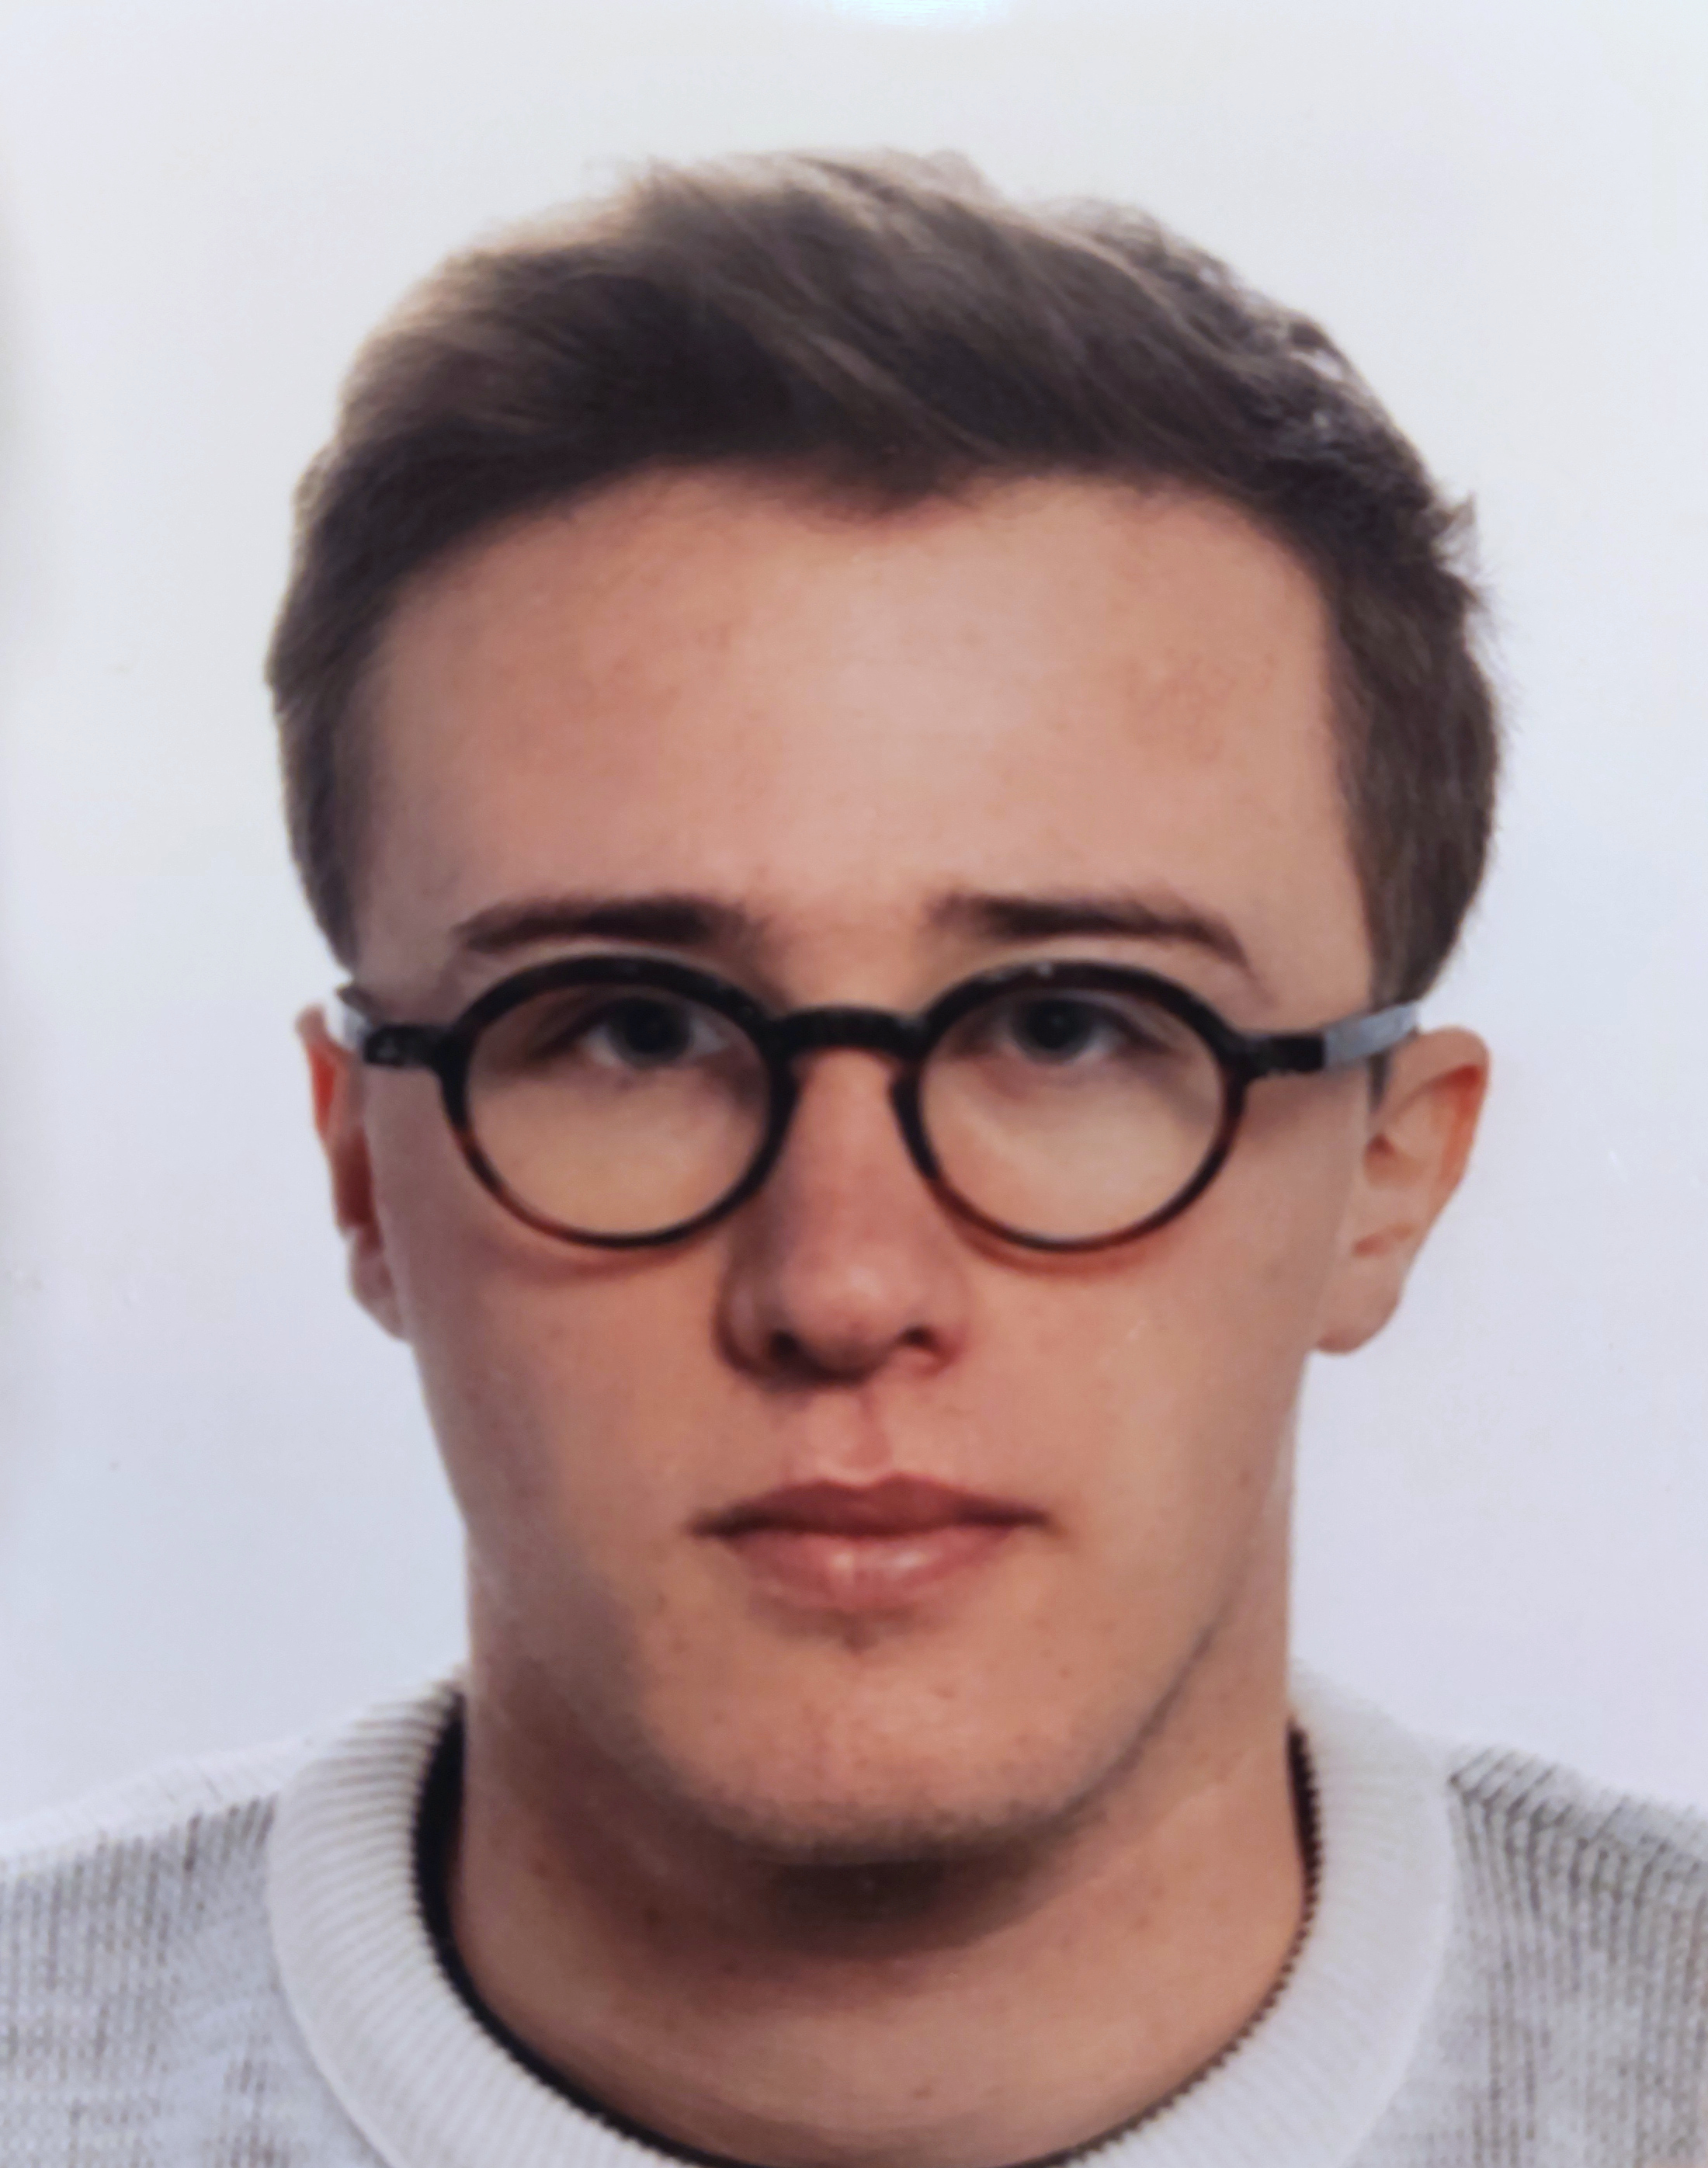
\includegraphics[width=\linewidth]{photo.jpg}
\end{minipage}


\section*{About me}

I am a Ph.D. candidate at KU Leuven Laboratory for Neuro- and Psychophysiology
and the University of Lille Research Center for Informatics, Signal Processing,
and Control Science. My research is centered on developing brain-computer
interface (BCI) technologies with a primary focus on assisting individuals with
severe disabilities, especially those with motor and eye movement impairments.
My goal is to enhance their quality of life by creating accurate and
user-friendly BCIs. Combining my expertise in machine learning, signal
processing, and user interface design with insights from neurophysiology, my
PhD centers around the development of an event-related potential BCI system
using EEG for real-time communication. I strongly believe in the potential of
innovative neurotechnology to empower individuals and patients, enabling them
to lead more independent and fulfilling lives.

\paragraph{Keywords:} brain-computer interfaces, event-related
potentials, multilinear classification, covert visual attention

\section*{Education}
\renewcommand{\arraystretch}{1.5}
\begin{tabularx}{\linewidth}{@{}p{1.2in} X@{}}
	ongoing & \makecell[{{X}}t]{
	\textbf{Ph.D. in Biomedical Sciences}, KU Leuven                                                         \\
	Supervisor: prof. Marc Van Hulle}                                                                        \\
	ongoing & \makecell[{{X}}t]{\textbf{Ph.D. in Control Science and Signal Processing}, University of Lille \\
	Supervisor: prof. François Cabestaing                                                                    \\
	}                                                                                                        \\
	2020    & \makecell[{{X}}t]{
	\textbf{M.Sc. in Engineering Science: Computer Science}, KU Leuven                                       \\
	Thesis: \textit{Linguistic transcription of EEG responses to sequences of visual stimuli}                \\
	Supervisor: prof. Marc Van Hulle                                                                         \\
	Major: Artificial Intelligence                                                                           \\
	Degree: \textit{cum laude}                                                                               \\
	}                                                                                                        \\
	2017    & \makecell[{{X}}t]{\textbf{B.Sc. in Informatics}, KU Leuven                                     \\
		% Thesis: \textit{Development of a quadcopter simulator and autopilot with stereoscopic object detection} \\
	Minor: Natural Sciences                                                                                  \\
	}                                                                                                        \\
\end{tabularx}

\section*{Publications}


\nocite{*}

\printbibliography[heading=none]


\section*{Awards}
\begin{tabularx}{\linewidth}{@{}p{1.2in} X@{}}
	30/11/2022 & \makecell[{{X}}t]{\textbf{NeuroTechX student club competition}, 4th place worldwide \\
		Our BrainBrowsR project, a plug-and-play BCI system that lets you control social media applications  trough SSVEP-BCI was awarded 90/100 points by the jury.}
\end{tabularx}


\section*{Funding}

\begin{tabularx}{\linewidth}{@{}p{1.2in} X@{}}
	01/2021 - 12/2024 & \makecell[{{X}}t]{\textbf{KU Leuven and University of Lille Global Ph.D. Partnership Grant} \\
	Topic: \textit{EEG-based visual brain-computer interface for gaze-free communication}.}                         \\
\end{tabularx}


\section*{Conferences and presentations}

\subsection*{Presented}

\begin{tabularx}{\linewidth}{@{}p{1.2in} X@{}}
	06/06/2023 & \makecell[{{X}}t]{\textbf{10th International BCI Meeting}, BCI
	Society                                                                     \\
		Poster presentation on classifier-based latency estimation for
	gaze-independent BCIs.}                                                     \\
	02/06/2022 & \makecell[{{X}}t]{\textbf{Leuven.AI Scientific Workshop
	2022}, Leuven.AI                                                            \\
		Poster presentation on (multi-)Kronecker-structured linear discriminant
	analysis for low sample size event-related potential classification.}       \\

	12/03/2022 & \makecell[{{X}}t]{\textbf{CORTICO 2022}, CORTICO               \\
		Presentation on Kronecker-structured LCMV-beamforming for event-related potential
	classification.}                                                            \\
	27/05/2021 & \makecell[{{X}}t]{\textbf{CORTICO 2021}, CORTICO              \\
		Presentation at CORTICO Young Researchers Day about a multi-component approach
	to spatiotemporal beamforming decoding of event-related potentials.}        \\
\end{tabularx}


\subsection*{Attended}

\begin{tabularx}{\linewidth}{@{}p{1.2in} X@{}}
  22/04 - 01/05/2024 & \makecell[{{X}}t]{\textbf{BCI \& Neurotechnology
  Spring School 2024}, g.tec} \\
	18/10 - 20/10/2023 & \makecell[{{X}}t]{\textbf{Closed Loop Neurotechnologies
  Autumn School}, NeurotechEU} \\
	09/05 - 10/05/2023 & \makecell[{{X}}t]{\textbf{CORTICO 2023}, CORTICO} \\
  17/04 - 26/04/2023 & \makecell[{{X}}t]{\textbf{BCI \& Neurotechnology
  Spring School 2023}, g.tec} \\
  28/09/2022 & \makecell[{{X}}t]{\textbf{BCI \& Neurotechnology Masterclass Belgium}, g.tec} \\
  25/04 - 04/05/2022 & \makecell[{{X}}t]{\textbf{BCI \& Neurotechnology
  Spring School 2022}, g.tec} \\
\end{tabularx}

\section*{Teaching Experience}

\subsection*{Classes}
\begin{tabularx}{\linewidth}{@{}p{1.2in} X@{}}
	02/2022 - ongoing & \makecell[{{X}}t]{\textbf{Teaching Assistant Brain-Computer Interfaces}, KU Leuven       \\
		Teaching exercise sessions in BCI design and
		signal processing to students in the Master of Bioengineering and
	Advanced Master of Artificial Intelligence.}                                                                 \\
	02 - 06/2020  & \makecell[{{X}}t]{\textbf{Student Assistant Fundamentals of Computer Science}, KU Leuven \\
		Teaching exercise sessions in Python programming and
		algorithmic reasoning to students in the Bachelor of
	Engineering Sciences.}                                                                                       \\
\end{tabularx}

\subsection*{Master theses and internships}
\begin{tabularx}{\linewidth}{@{}p{1.2in} X@{}}
	2023 - 2024       & \makecell[{{X}}t]{\textbf{Linear Discriminant Analysis in
	the combined space-time-frequency domain for BCI decoding}, \textit{Yildiz
  Dilara}
Parry, KU Leuven}                                                                          \\
	2023 - 2024       & \makecell[{{X}}t]{\textbf{Tackling the Midas Touch
  problem in eye tracking with a BCI}, \textit{Lunkyadi Sucipto}, KU Leuven}                                                                                                 \\
	2023 - 2024       & \makecell[{{X}}t]{\textbf{A connectivity-based EEG
  analysis of Alzheimer’s Disease and Frontotemporal Dementia}, \textit{Zoe
Barinaga}, KU Leuven} \\
	02 - 06/2024       & \makecell[{{X}}t]{\textbf{Eye-tracker and ERP data
    fusion for gaze-independent visual BCI}, \textit{Juliette
  Meunier}, Université de Lille} \\
	03 - 05/2023 & \makecell[{{X}}t]{\textbf{Single-trial ERP component latencies as a predictor for the mode of visual attention}, KU Leuven} \\
	2021 - 2022       & \makecell[{{X}}t]{\textbf{A hybrid P300-gaze BCI alternative
  for navigating in Virtual spaces}, \textit{Gijs Claes}, KU Leuven}                                                                                                   \\
\end{tabularx}


\subsection*{Extracurricular}
\begin{tabularx}{\linewidth}{@{}p{1.2in} X@{}}
	05/2022 - ongoing & \makecell[{{X}}t]{\textbf{Project supervisor}, NeuroTech Leuven                          \\
		Project supervisor and technical advisor for extracurricular
	neurotechnology student projects and a student team participating in the annual NeuroTechX BCI competition.} \\
	09/2015 - 01/2016 & \makecell[{{X}}t]{\textbf{PAL tutor Principles of Computer Programming}, KU Leuven       \\
		Organizing and teaching peer-assisted learning sessions in Python programming for first year informatics
	students.}                                                                                                   \\
\end{tabularx}

\section*{Professional and volunteering Experience}

\begin{tabularx}{\linewidth}{@{}p{1.2in} X@{}}
	2022 - ongoing    & \makecell[{{X}}t]{\textbf{Ambulance EMT}, Red Cross, FAST
	vzw}                                                                                                \\
	07 - 12/2019 & \makecell[{{X}}t]{\textbf{Python developer}, Mindspeller                        \\
		Python Flask developer in a KU Leuven spin-off that provides neuromarketing services based on
		scientifically validated neuroscience and
	AI research.}                                                                                       \\
	2014 - 2020       & \makecell[{{X}}t]{\textbf{Freelance full-stack web
	developer}, Self-employed}                                                                          \\
	%2018 - 2019       & \makecell[{{X}}t]{\textbf{Board Secretary}, Scientica Leuven vzw}               \\
	%2015 - 2020       & \makecell[{{X}}t]{\textbf{Webmaster}, Wina Leuven vzw and Scientica Leuven vzw} \\
	%2013 - ongoing    & \makecell[{{X}}t]{\textbf{Event EMT}, Red Cross}                                \\
\end{tabularx}


\section*{Licenses and certifications}
%\begin{tabularx}{\linewidth}{@{}p{1.2in} X@{}}
%	2022 & \makecell[{{X}}t]{\textbf{Ambulance EMT}, FOD
%	Volksgezondheid}                                                 \\
%	2021 & \makecell[{{X}}t]{\textbf{ICH Good Clinical Practice E6},
%	TransCelerate BioPharma Inc. }                                   \\
%\end{tabularx}

\textbf{ICH Good Clinical Practice}, E6 TransCelerate BioPharma Inc.
\smallskip

\textbf{Ambulance EMT}, FOD Volksgezondheid \\

\section*{Languages}
\begin{tabularx}{\linewidth}{@{}p{1.2in} X@{}}
	Dutch   & Native           \\
	English & Fully proficient \\
	French  & Advanced         \\
	German  & Intermediate     \\
\end{tabularx}




\end{document}
